% KU defaults
\documentclass[11pt, a4paper]{article}
\usepackage[english, science, titlepage, dropcaps]{ku-frontpage}
\usepackage[utf8]{inputenc}

% Additional packages
\usepackage{lipsum}
\usepackage{cite}
\usepackage[toc,page]{appendix}

% KU settings
\setlength\arraycolsep{2 pt}
\setcounter{tocdepth}{2}
\setcounter{secnumdepth}{0}

% User settings

\assignment{Master thesis}
\author{Martin Thiele}

\title{Banking the unbanked}
\subtitle{Utilizing current technology to bank the unbanked to support the transition from cash to online payment}
\date{Handed in: \today}
\advisor{Advisors: Fritz Henglin, Søren Terp}
\frontpageimage{example.png}

\begin{document}

\renewcommand{\bibname}{References}


\maketitle

\begin{abstract}
\lipsum[1]
\end{abstract}

\clearpage

\section*{Acknowledgements}
\lipsum[2]

\clearpage

\tableofcontents
\clearpage


\section{Introduction}

% Introduce the problem and why banking is necessary
Financial inclusion is the ability to have access to basic banking which includes efficient and secure transactions, trusted ownership, execution of payments, safe storage of money, and withdrawal of cash. This has been defined by The World Bank to be an important building block for both poverty reduction and opportunities for economic growth\cite{gfindex} and is one of the focal points of many international agencies, such as the International Monetary Fund (IMF)\footnote{\url{https://www.imf.org/en/About/Factsheets/IMF-at-a-Glance}} and The World Bank\footnote{\url{https://www.worldbank.org/en/what-we-do}}, as well as non-profit organizations (NPOs) like the Norwegian Refugee Council (NRC)\footnote{\url{https://www.nrc.no/what-we-do/themes-in-the-field/cash-and-vouchers/}}. By having access to these tools societies will see many benefits. In Niger, a five-month relief program swapped from a monthly payment of cash to instead use mobile money services allowing for mobile commerce (m-commerce). This change saved the recipients 20 hours on average in overall travel and wait time to obtain the payments\cite{gfindex}. A similar study was performed in Kenya where the change to mobile money services allowed 185,000 women-headed households to increase their savings by more than 20 \%, reducing extreme poverty among these households by 22 \%. Additionally, access to digital payments allows for easier storage and a reduction in corruption in countries where trust in the government is low\cite{gfindex}.

% Statistics
% Statistics - Amount of banked / unbanked
\begin{figure}[ht]
\centering
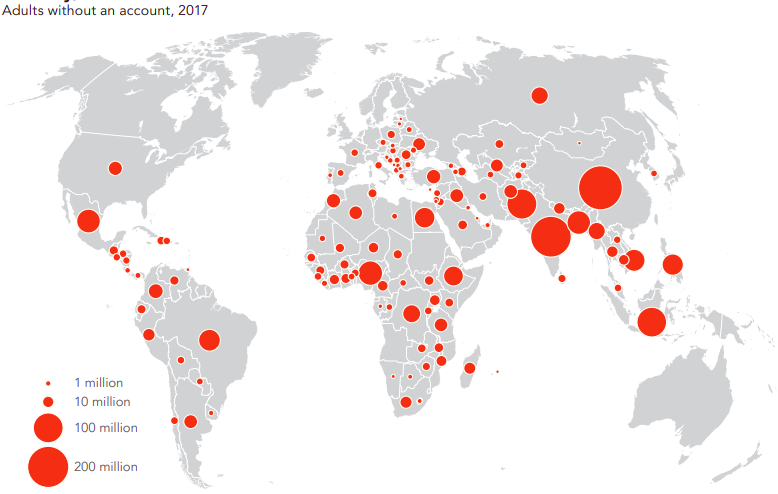
\includegraphics[width=1\linewidth]{figs/unbanked_map}
\caption{\textit{The Global Findex Database}. Map of locations for unbanked adults in 2017.}
\label{fig: unbanked_map}
\end{figure}


The Global Findex Database reports that 69 \% of adults in 2017 had a bank account\cite{gfindex}, an increase of 7 \% since 2014 and 18 \% since 2011\cite{gfindex}. 94 \% of adults in developed countries own a bank account, whereas only 63 \% of adults own an account in developing countries\cite{gfindex}. Globally, approximately 1.7 billion adults remain unbanked, with half of them living in just seven developing areas: Bangladesh, China, India, Indonesia, Mexico, and Pakistan. Furthermore, we can from \autoref{tab:financial_statistics} and \autoref{fig: unbanked_map} deduce that majority of the financially excluded people are located in the Middle East \& North Africa (43.5\%), and Sub-Saharan Africa (SSA) (42.6\%), whereas only 32.8\% of the people in SSA are banked through traditional means. 20.9\% are banked through mobile money accounts showing how mobile money is already blossoming in this region.


\begin{table}[!ht]
\begin{tabular}{|l|l|l|l|}
\hline
\textbf{Region}             & \textbf{Account (\%)} & \textbf{FI account (\%)} & \textbf{M\footnote{Mobile money account} (\%)} \\ \hline
East Asia \& Pacific        & 70.6                  & 70.3                     & 1.3                                \\ \hline
Europe \& Central Asia      & 65.3                  & 65.1                     & 3.2                                \\ \hline
Latin American \& Caribbean & 54.4                  & 53.5                     & 5.3                                \\ \hline
Middle East \& North Africa & 43.5                  & 43.0                     & 5.8                                \\ \hline
South Asia                  & 69.6                  & 68.4                     & 4.2                                \\ \hline
Sub-Saharan Africa          & 42.6                  & 32.8                     & 20.9                               \\ \hline
\end{tabular}
\caption{Financial inclusion statistics from six regions of the world, aged 15 and up\cite{littledata}}.
\label{tab:financial_statistics}
\end{table}

Throughout this thesis, we will be focusing on SSA since this region is in the largest need of financial inclusion, is more susceptible to outside support, and has had more research done and data on the topics of financial inclusion and mobile money.

Typical reasons for why the people in SSA are unbanked are noted in \autoref{tab:ssa_reasons}.
% Reasoning for being unbanked
\begin{table}[!ht]
\begin{tabular}{|l|l|}
\hline
\textbf{Reason} & \textbf{Surveyed who list it as a reason (\%)}\\ \hline
Distance to bank & 27 \\ \hline
Services are too expensive & 27 \\ \hline
Lack of necessary documentation & 25\\ \hline
Lack of trust in financial institutions & 14 \\ \hline
Religious reasons & 4 \\ \hline
Insufficient funds & 73 \\ \hline
A family member has an account & 11 \\ \hline
\end{tabular}
\caption{Reasons for lack of financial accounts in Sub-Saharan Africa\cite{gfindex}}
\label{tab:ssa_reasons}
\end{table}

To further expand on the reasonings from \autoref{tab:ssa_reasons}. The people of countries in SSA reason their lack of a financial account with 27\% of them citing the distance is a problem. Particularly in the rural areas of SSA, travel to banks is too big a reliability, especially in countries where the GDP is so little that most payments are considered micropayments ($< \$1$).

Another common issue is the lack of documentation which 25\% cite as reasoning, making the person too big of a risk for traditional banks to consider. 14\% denote the lack of trust in financial institutions. Trust is an important factor for any business and it is particularly the countries who lack trust in their government who also lacks trust in financial institutions, notable countries such as the Democratic Republic of Congo (DRC) (26\%)\cite{gfindex} who has had a long history of corruption, and Central African Republic (CAR) (24\%)\cite{gfindex} who is in the middle of a civil war, suffer from constant instability and is ranked 1 on the global hunger index\cite{ghi}.

Many countries in SSA are highly religious but only a few of them list religion as a concern. Niger is a Muslim-dominant country with 98.4\% of the population being M-Pesauslim\cite{muslim}. Islamic finance comes with a set of rules which should be in accordance with Islamic law, particularly lending with interest is prohibited because it is deemed exploitative to earn money from interest\cite{islam_invest}.

11\% cite that they don't have an account because a family member has one, this can be explained by the service cost of being banked, or because of financial literacy issues. In general, the amount of education in SSA is very low with some countries having less than two years of schooling on average\cite{hdr}.



% Statistics - mobile phones / internet
When looking at developing countries and financial technology (fintech) it is important to consider what technologies are available in these areas. 1.1 billion of the financially excluded adults own a mobile phone\cite{gfindex}, however, many developing countries have very little internet access. Our World in Data reports that for the majority of the countries in SSA, the population with access to the internet are only between 5 and 20 \%\cite{owidinternet}, however for most of these countries, the mobile phone penetration rate\footnote{The mobile phone penetration rate refers to the amount of SIM cards in a certain country} is greater than 40 \%\cite{owidinternet}. The mobile network is more advanced than most would probably imagine. 80\% of rural Africa is covered, with 22\% of it being 4G, 40\% being 3G and 18\% being 2G. Urban Africa is fully covered with 77\% 4G and 23\% 3G\cite{ituinternet}. The average download speed in this area has increased from 0.5 Mbps in 2014, to 2.4 Mbps in 2017\cite{gsma}. 100MB of network data costs on average 4.3\% of the monthly GDP per capita, a decrease from 2014s 8.6\%. This is fairly expensive, but the halving in cost in just three years shows the promising future mobile phones have, and will have in this region.


Banking the unbanked is a \$380 billion revenue opportunity\cite{accenture} which has seen an increase in interest throughout the last decade, mainly due to the success M-Pesa has had in Kenya. M-Pesa is a mobile phone-based money transfer service launched in 2007 by the telecommunications company Vodafone Group and the mobile network operator (MNO) Safaricom. M-Pesa utilizes the Unstructured Supplementary Service Data (USSD), also known as "quick codes", a protocol similar to short message service (SMS) with the exception that it creates a connection allowing for a two-way exchange between the parties. Additionally, it doesn't store the messages on the mobile phone. The benefit of using USSD is that it is a feature available in both smartphones and dumbphones\footnote{A mobile device without internet capacity ad little computing power}, making it available to every user with a mobile phone. With a mobile phone penetration rate of 103.769\cite{wbinternet}, it is safe to assume that most of the citizens are covered. {\color{red} Continue explaining the success of M-Pesa, or move to a different section? Or discard.}\\


Throughout this thesis we will take an example-driven approach of defining the needs and requirements of a mobile banking application, as well as determine the best country to onramp such a project, ensuring that the targeted country's needs, likewise, are met. When the requirements are defined we will implement a basic bank meeting these requirements, utilizing the technology that is available to them, with features that allow for any user to see the benefits of entering the mobile bank network. We will then evaluate the use cases of this product, measured up against existing mobile banks, before performing a security analysis looking at the potential attack vectors of the mobile bank. We will then discuss the implementation and reason for our choices before taking a look at the existing work done within this field which we have drawn inspiration from, as well as note what we find, could be a useful next step if this project were to be developed further. Finally, we will conclude with our findings.







\section{Technical chapter}
What needs its own section to cover? How we settled on Guinea? Why we ended up workin with USSD/Android? Obtaining trust? The story of M-Pesa?
\section{Technical chapter 2}

\section{Proposed architecture}
\subsubsection{Design}
\subsection{Server} % (fold)

\subsubsection{Database}
\subsubsection{USSD API}
\subsubsection{Android API}
% subsection server (end)
\subsection{Android}
% subsection android (end)

\section{Evaluation}
\section{Discussion}
\subsection{Related work} % (fold)
\label{sub:related_work}

% subsection related_work (end)
\subsection{Future work} % (fold)
\label{sub:future_work}

% subsection future_work (end)

\subsubsection{Pre-commit} % (fold)
\label{sub:pre_commit}
The implementation currently works in 3 stages.
\begin{enumerate}
    \item A request is made for one person to send money to the other.
    \item the requested person and the requesting person meet and trades the cash.
    \item The requested person confirms the request in 1.
\end{enumerate}
This implementation does not take into account whether the requestee has the funds to finish the transfer. A pre-commit would be in order to prove that there is a sufficient amount of funds, thereby reducing theft opportunities.
% subsubsection pre_commit (end)
\subsubsection{Blockchain technology} % (fold)

\label{sub:blockchain_technology}
{\color{red} Move to discussion instead}

From {\color{red} section xx} we determined that a E-money license costs {\color{red} xx}, due to the unregulated nature of cryptocurrency it might be easier to work with cryptocurrencies instead. There are additional benefits to this.
\begin{enumerate}
    \item Stablecoins (cryptocurrency typically pegged to the US Dollar) can allow for people in fluctuating economies to enter a stable one.
    \item Cryptocurrency is currently a popular means of investing and is being sought by multiple people.
    \item Cryptocurrencies allow for easy cross-border transfers.
\end{enumerate}
% subsubsection blockchain_technology (end)
\section{Conclusion}

\begingroup
\let\cleardoublepage\clearpage
\bibliographystyle{acm}
\bibliography{thesis}
\endgroup

\begin{appendices}
\section{Source code}
\section{Copyright attribution}
The icons used for the android application is part of the Finance Icons package by the Noun Project, licensed under the CC BY 4.0 license. To view the icon package, visit \url{https://thenounproject.com/term/finance/}. To view the terms of the license, visit \url{https://creativecommons.org/licenses/by/4.0/}
\end{appendices}
\end{document}